%%%%%%%%%%%%%%%%%%%%%%%%%%%%%%%%%%%%%%%%%%%%%%%%%%%%%%%%%%%%%%%%%%%%%%%%%%%%%%%
%% StuPro B, "Programmierumgebung Offener Antrieb" (POA)
%% Entwurf
%% $Id: format.tex,v 1.1 2004/05/18 23:51:49 vanto Exp $
%% Achtung: Diese Datei wird in den Entwurf inkludiert!
%%%%%%%%%%%%%%%%%%%%%%%%%%%%%%%%%%%%%%%%%%%%%%%%%%%%%%%%%%%%%%%%%%%%%%%%%%%%%%%

\chapter {Einleitung}
Dieses Dokument beschreibt das Format der POA Projektdateien. Diese
Dateien werden im XML-Format im Projektverzeichnis abgelegt.

Die Datei gliedert sich auf h�chster Ebene in zwei Teile, die von dem
Wurzelelement umschlossen werden. Der erste Teile repr�sentiert das
Datenmodell, der zweite Teil bezieht sich auf die Darstellung der
Bl�cke. Diese View-Elemente beziehen sich �ber eine ID auf den
jeweiligen Block im Modell-Bereich. Eine Ausnahme bilden hier die
Verbindungen zwischen Bl�cken. Diese haben keine Modellinstanz sondern
werden nur als View-Element abgespeichert.

Die folgende Abbildung verdeutlicht den Aufbau der Projektdatei.

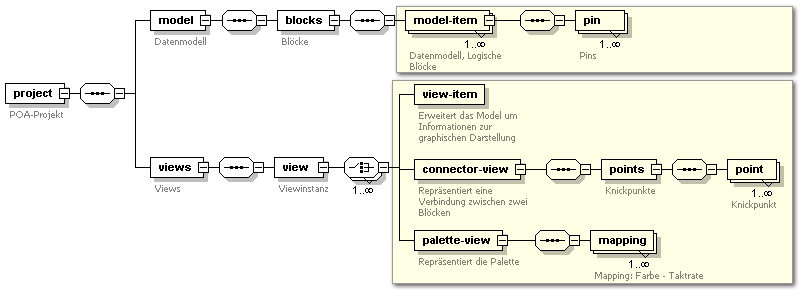
\includegraphics[width=16cm]{poa-schema}

\chapter{Struktur}
%TODO: weird table stuff

\chapter{Daten}
%TODO: weird table stuff

\chapter{Anhang A - DTD}
\chapter{Anhang B - XSD}

%%% Local Variables: 
%%% TeX-master: "xmldoku"
%%% End: 
%%% vim:tw=79:
